
%% bare_jrnl_compsoc.tex
%% V1.3
%% 2007/01/11
%% by Michael Shell
%% 04/05/10
%% Edited by Suleyman Muhammad
%% See:
%% http://www.michaelshell.org/
%% for current contact information.
%%
%% This is a skeleton file demonstrating the use of IEEEtran.cls
%% (requires IEEEtran.cls version 1.7 or later) with an IEEE Computer
%% Society journal paper.
%%
%% Support sites:
%% http://www.michaelshell.org/tex/ieeetran/
%% http://www.ctan.org/tex-archive/macros/latex/contrib/IEEEtran/
%% and
%% http://www.ieee.org/
\documentclass[11pt,onecolumn,cspaper,compsoc]{IEEEtran}

% *** GRAPHICS RELATED PACKAGES ***

\usepackage{graphicx,color}
\graphicspath{{/home/suleyman/LaTex/pics/}}

\DeclareGraphicsExtensions{.eps, .pdf, .png, .jpeg}

\renewcommand{\thesection}{\Roman{section}}
\renewcommand{\thesubsection}{\thesection.\roman{subsection}}

\def\subsize{\@setsize\subsize{14pt}\xipt\@xipt}

\begin{document}
\title{Dynamic Source Routing Implementation}

\author{John Hashem\\\and John Roland\\\and Suleyman Muhammad\\\and Todd Matzelle\\\and Ying Jin}

% The paper headers
\markboth{ECE 8408-001: Mobile Computing \& Wireless Networks, December~2010}%
{MOB \MakeLowercase{\textit{et al.}}: ECE 8408}

\IEEEcompsoctitleabstractindextext{%
\begin{abstract}
The purpose of this project is to demonstrate a practical implementation of the Dynamic Source Routing (DSR) algorithm, or variance thereof, within a real life environment. The routing program has been written in C for a Linux environment and can be run from the command line. With our implementation of the DSR protocol, we utilized Nokia N800 tablets as nodes for routing.  At the beginning of the message transmission, the route discovery protocol is used to find the route; each node has a route cache in which it can cache source routes that it has learned. Message transmission following route cache works before route cache expired.  If any node fails or runs out of power, the route maintenance protocol will take effect and the new route will be found through the route discovery process.
\end{abstract}
}
% make the title area
\maketitle


\section{Introduction}

In ad-hoc networks, a collection of mobile nodes within wireless transmission range of one another may form a temporary network without the aid of any infrastructure or centralized administration. With the formation of these ad-hoc networks, the exchange of information often spans across multiple nodes.  As such, multi-hop routing protocols are most appropriate for use.  For our project, the Dynamic Source Routing (DSR) protocol was selected and implemented as a modified version of the algorithm. This protocol is reactive and requires no periodic advertisements for the discovery or maintenance of routes. Instead, functions are performed in an on-demand manner where sending nodes only request routing information when an entry to a destination does not exist within its own cache.  Whether already in cache or built in an on-demand manner, a complete sequence of nodes (network hops) is be provided. This sequence of nodes is used to forward a packet to its targeted destination.  Due to the on-demand nature of requests, overhead is often largely reduced. This is especially the case when little or no significant host movement is taking place.   

\section{Design Process}

The design process began with the creation of a state machine, which first depicted the traditional implementation of the DSR algorithm.  Utilizing this as a basic framework for our design, each of the processes of the algorithm was designed, built, and implemented.  Any variations from DSR were then mirrored in changes made to our final version of the modified DSR state machine diagram.  In our design we determined that four kinds of message packets were necessary: Data, Route Request, Route Reply, and Error.  The formats of these packets differ from the traditional DSR implementation, which is explained in more detail later in this document.  Branches of the state machine began as pseudo-code and were then implemented in the C programming language.  Code was written on the Linux operating system and compiled using the GNU C compiler (gcc).  Additionally, compilation was done in the Scratchbox environment in order to simulate the N800’s processor.

\newpage

\subsection*{Deviations from Traditional DSR Protocol}

As mentioned above, during the design of our protocol modifications were made to the original DSR algorithm.  These changes include; transmitting messages back to the sender with an error, having the sending node handle Route Requests resulting from errors, and changing the overall format of packets.

\subsection*{Modified DSR State Machine Diagram}

The state machine below illustrates the high level decision making process from the perspective of any given node within a wireless ad-hoc network.  As shown below, information exchanges for nodes will always start and end within the \emph{Wait} state.  Each rectangle represents a unique state, while arrows highlight events/actions that are taken.  Please note that thick lines denote the 1st events/actions taken after the \emph{Wait} state.

\begin{figure}[!h]
  \centering
  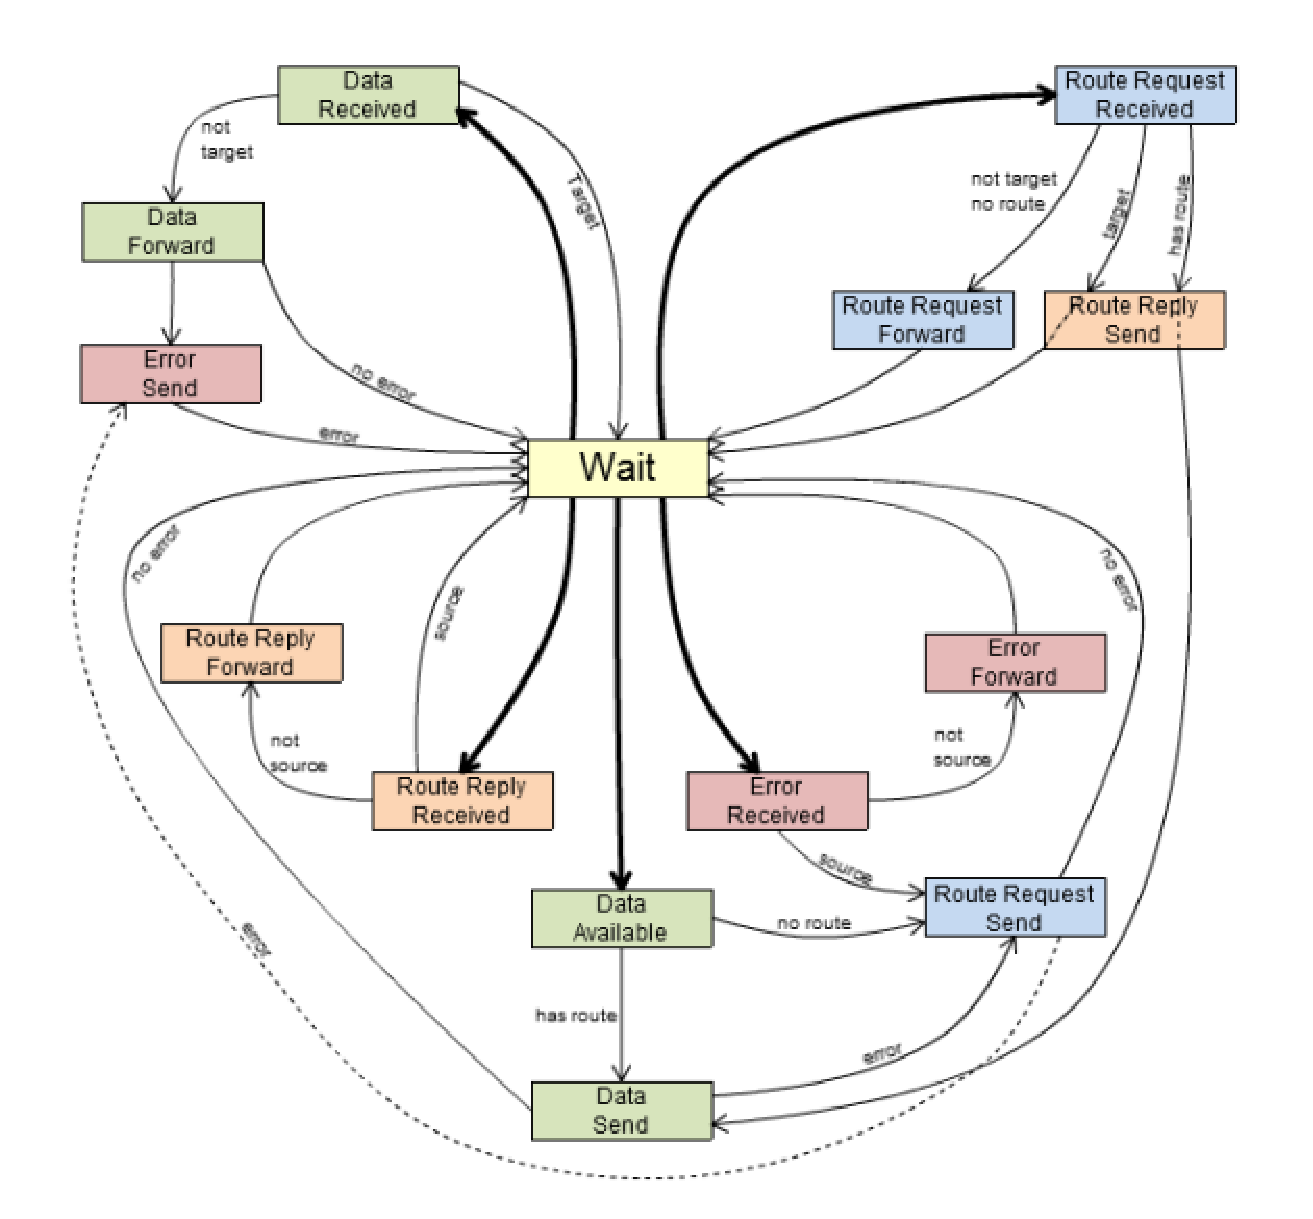
\includegraphics[scale=.6]{DSR_State}
  \caption{DSR State Machine Diagram}
  \label{DSRSM}
\end{figure}

\newpage

\subsection*{Modified DSR Path Permutations Chart}

The following chart illustrates all unique permutations of events/actions and states that can occur using the modified DSR state diagram.  For spatial reasons, the original chart was simplified so that it could be included within this document.  If desired, the complete chart is available as an appendix to this paper.

This chart is a good example how a quality assurance engineer might attack testing our algorithm, and serves as a measurable and reportable format for communicating results back to a developer.  In our case the chart serves to illustrate how many scenarios can occur, in what order, and beginning with what state and shows where certain permutations would fail is functions are incomplete.  While reviewing the chart please note that all colors correlate directly with states within the state diagram.

\begin{figure}[!h]
  \centering
  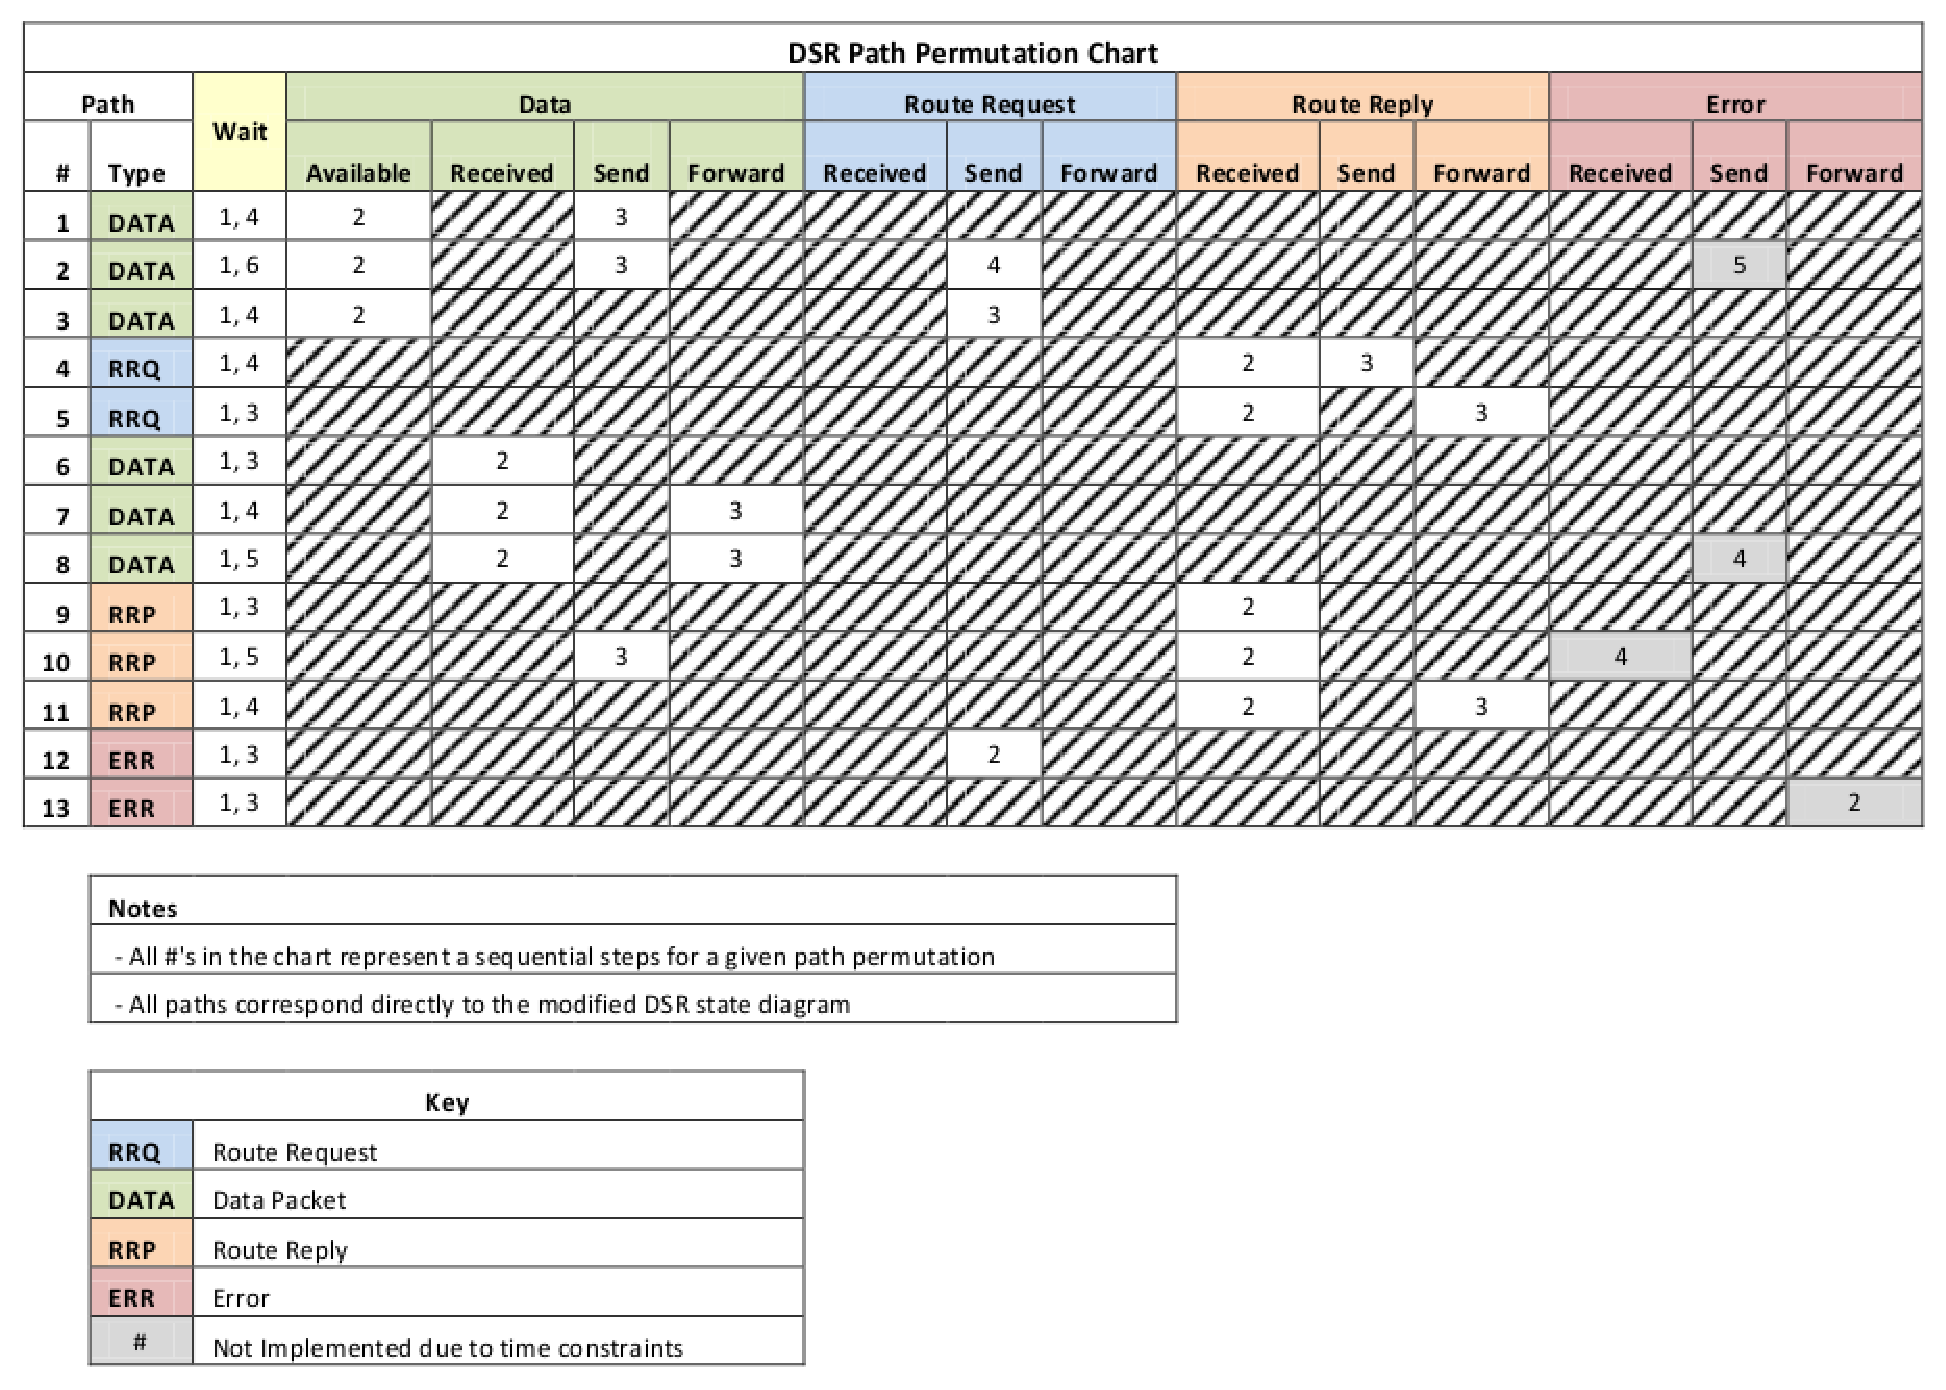
\includegraphics[scale=.5]{DSR_path}
%  \caption{DSR Path Permutation Chart}
  \label{DSR Path}
\end{figure}

\newpage

\subsection*{Packet Formats}

The following tables represent various packet formats utilized for communication between nodes, using our modified DSR algorithm. 

\begin{figure}[!h]
  \centering
  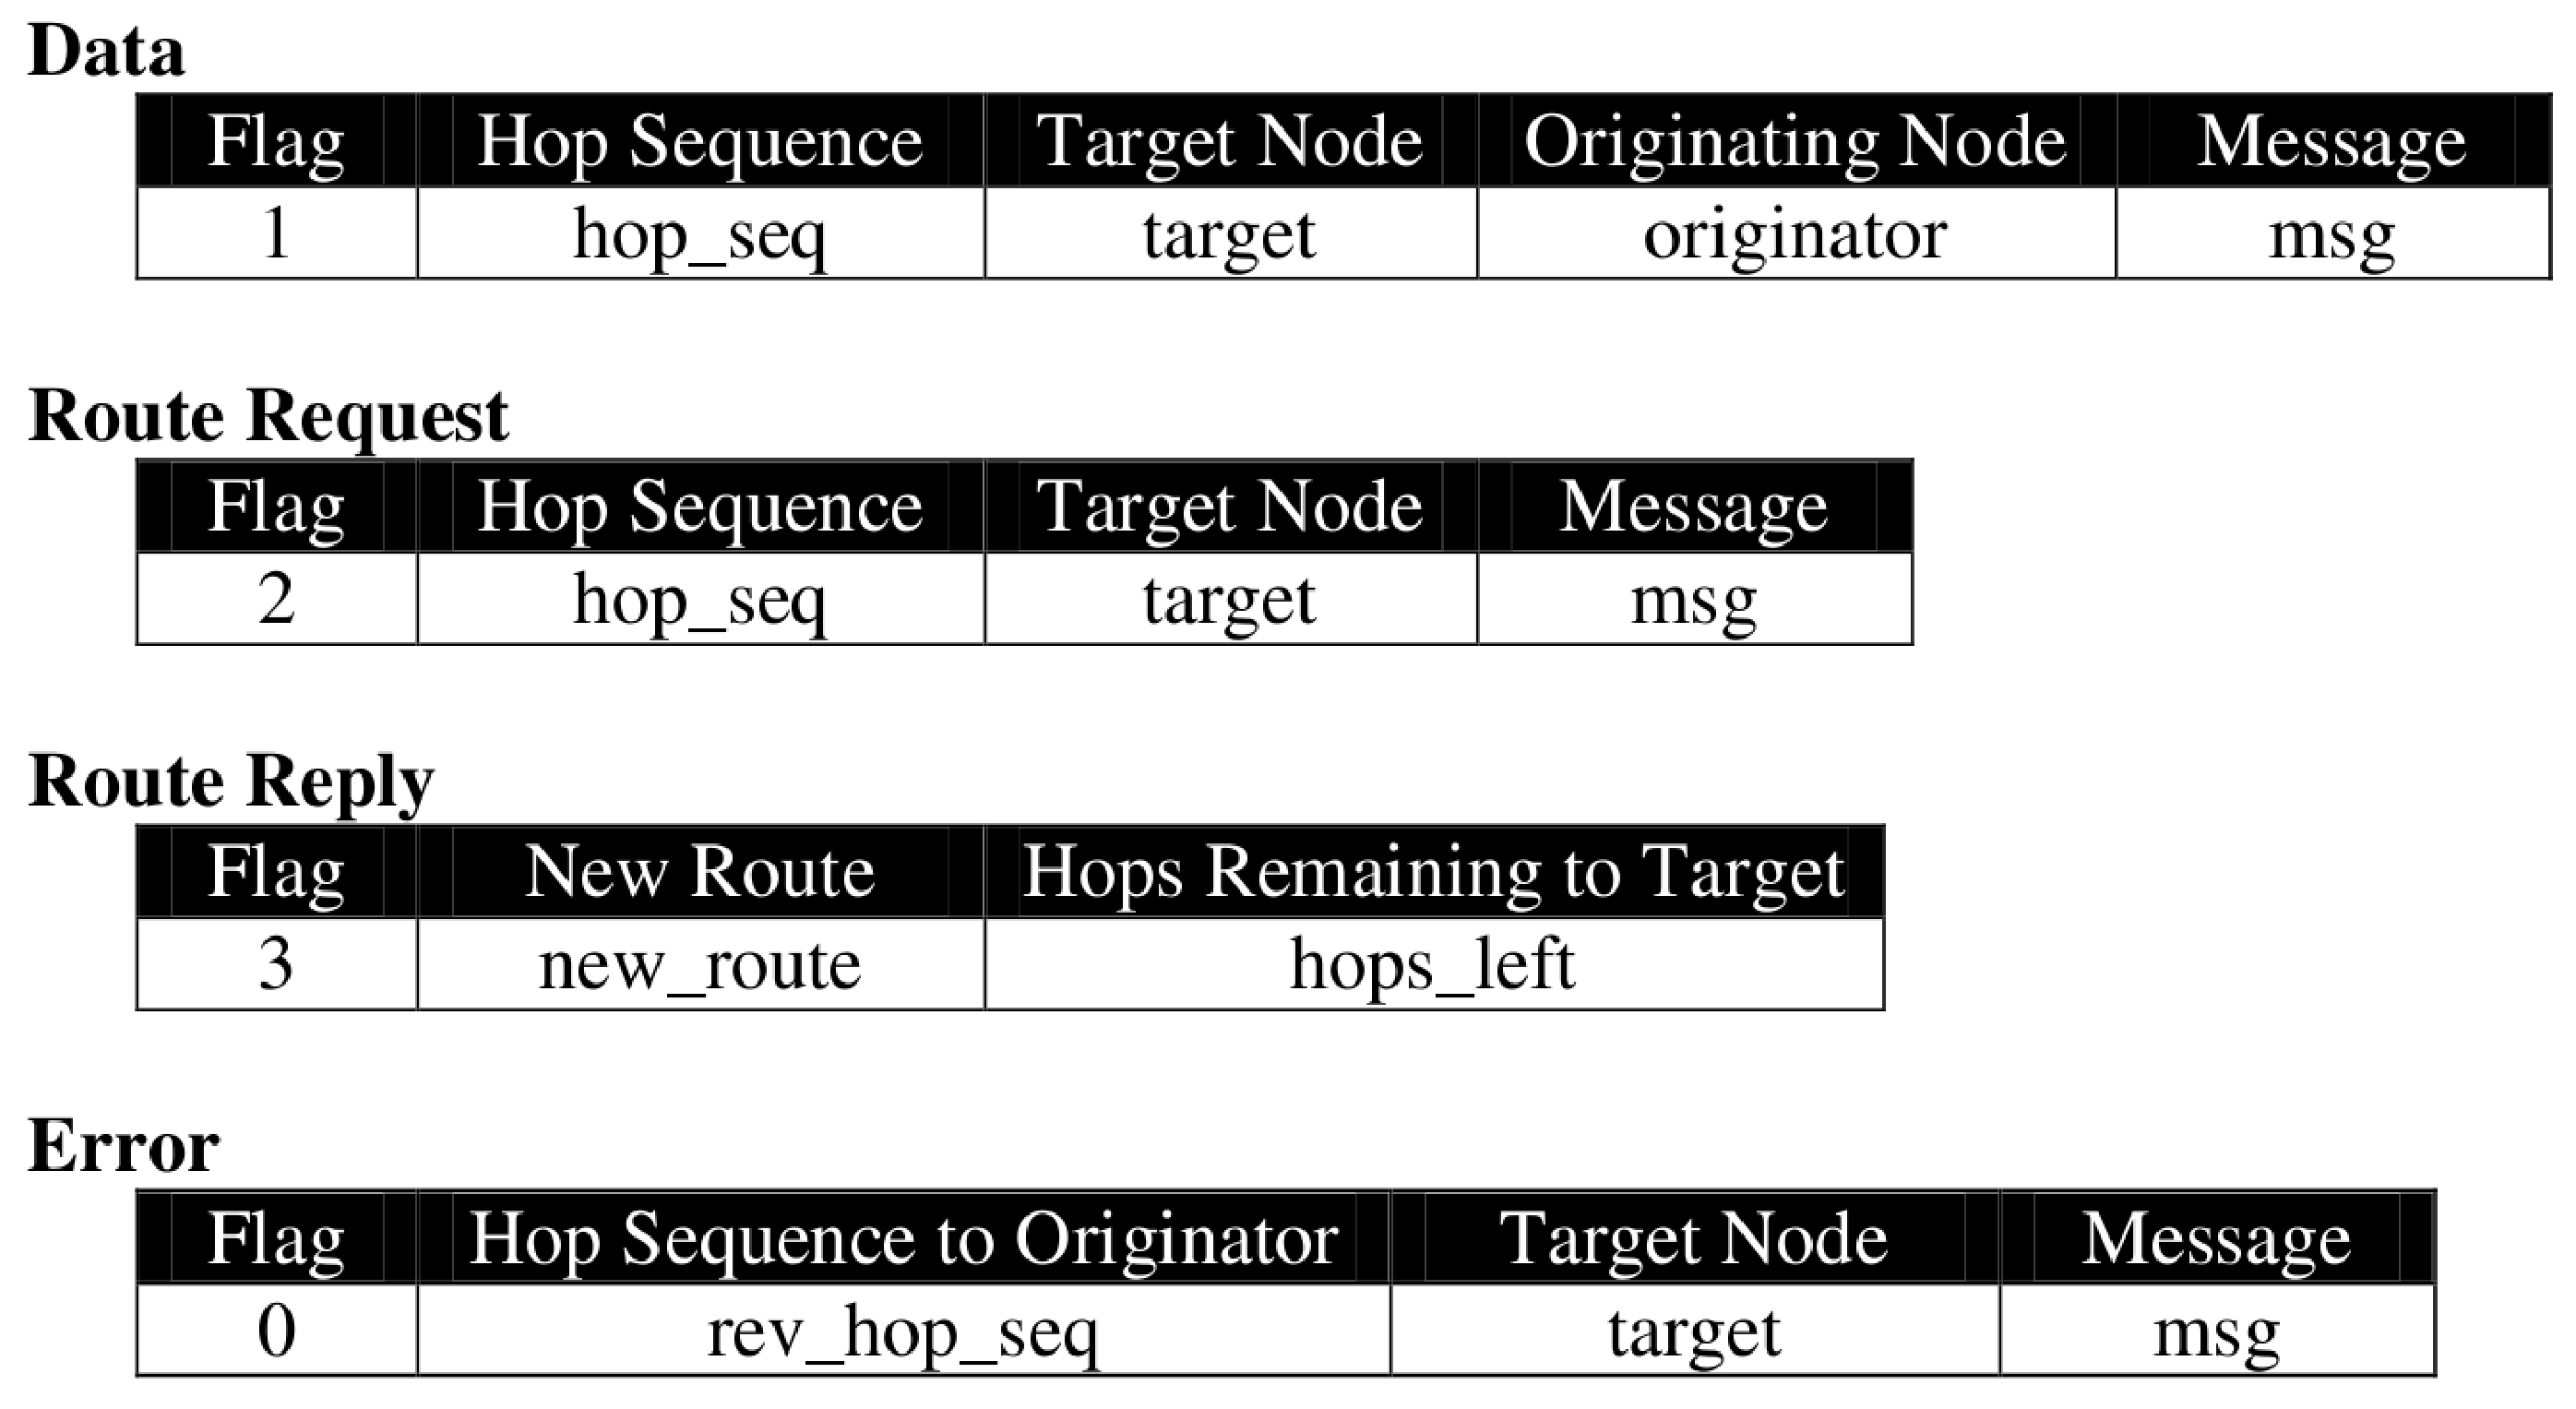
\includegraphics[scale=.25]{Packet}
%  \caption{Packet}
\end{figure}

\subsection*{Hop Sequence Format}

The “hop\_seq” in the above packet formats is a semi-colon-delimited string containing all of the hops that a message must take to get to its destination.  The table below illustrates this format and the process by which a hop sequence is rotated.  Changes in hop sequence occur each time a packet is passed from one node to another.

\begin{figure}[!h]
  \centering
  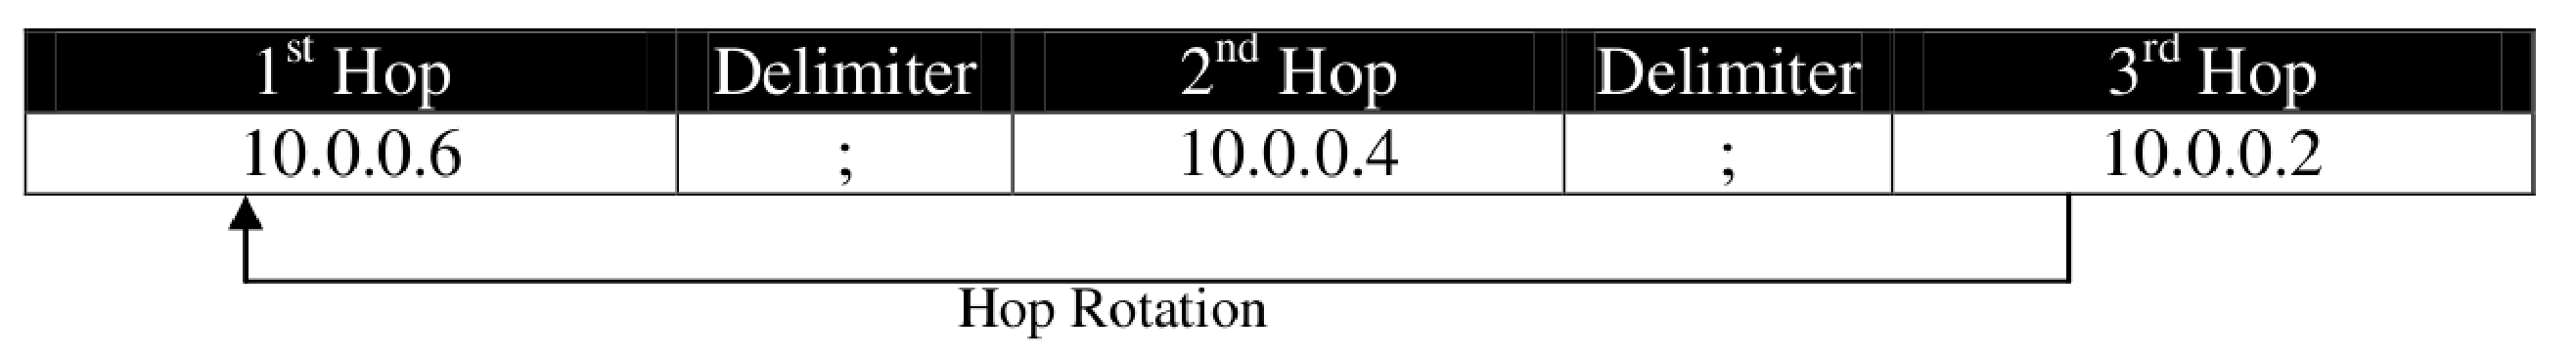
\includegraphics[scale=.3]{Hop_Seq}
%  \caption{Hop Sequence}
  \label{Packet}
\end{figure}

\subsection*{Simulation Example}

The following is an example of how our simulation works using the packet formats mentioned above. Please note that the colors used below do \emph{not} correlate with the state diagram or DSR path permutations chart.

Here’s a breakdown of the details surrounding this message:

\begin{figure}[!ht]
  \centering
  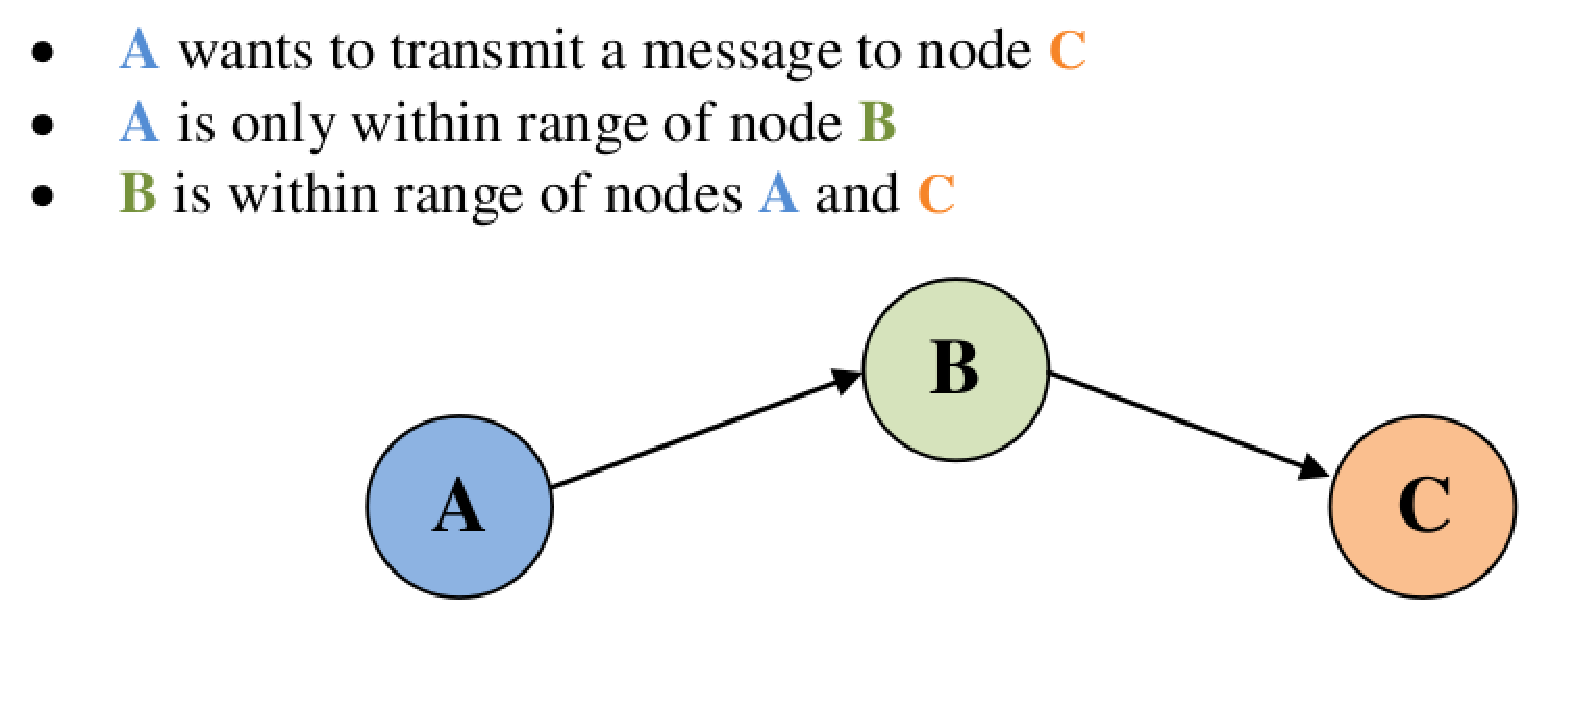
\includegraphics[scale=.4]{Route}
%  \caption{Route A to C}
  \label{route}
\end{figure}

\newpage

\subsection*{Assumtions}

\begin{itemize}
 \item \color{blue}{A} \color{black}{has already moved from the \emph{Wait} state to \emph{Data Available} and is now ready to try and send data}.
 \item \color{blue}{A} \color{black}{realizes that it has no route entry for a path to the target node.}
 \item \color{blue}{A} \color{black}{knows that it must follow the process below in order to obtain this missing route.}
\end{itemize}

\subsection*{The Route Request (RRQ) \& Route Reply (RRP) Process}

\begin{figure}[!h]
  \centering
  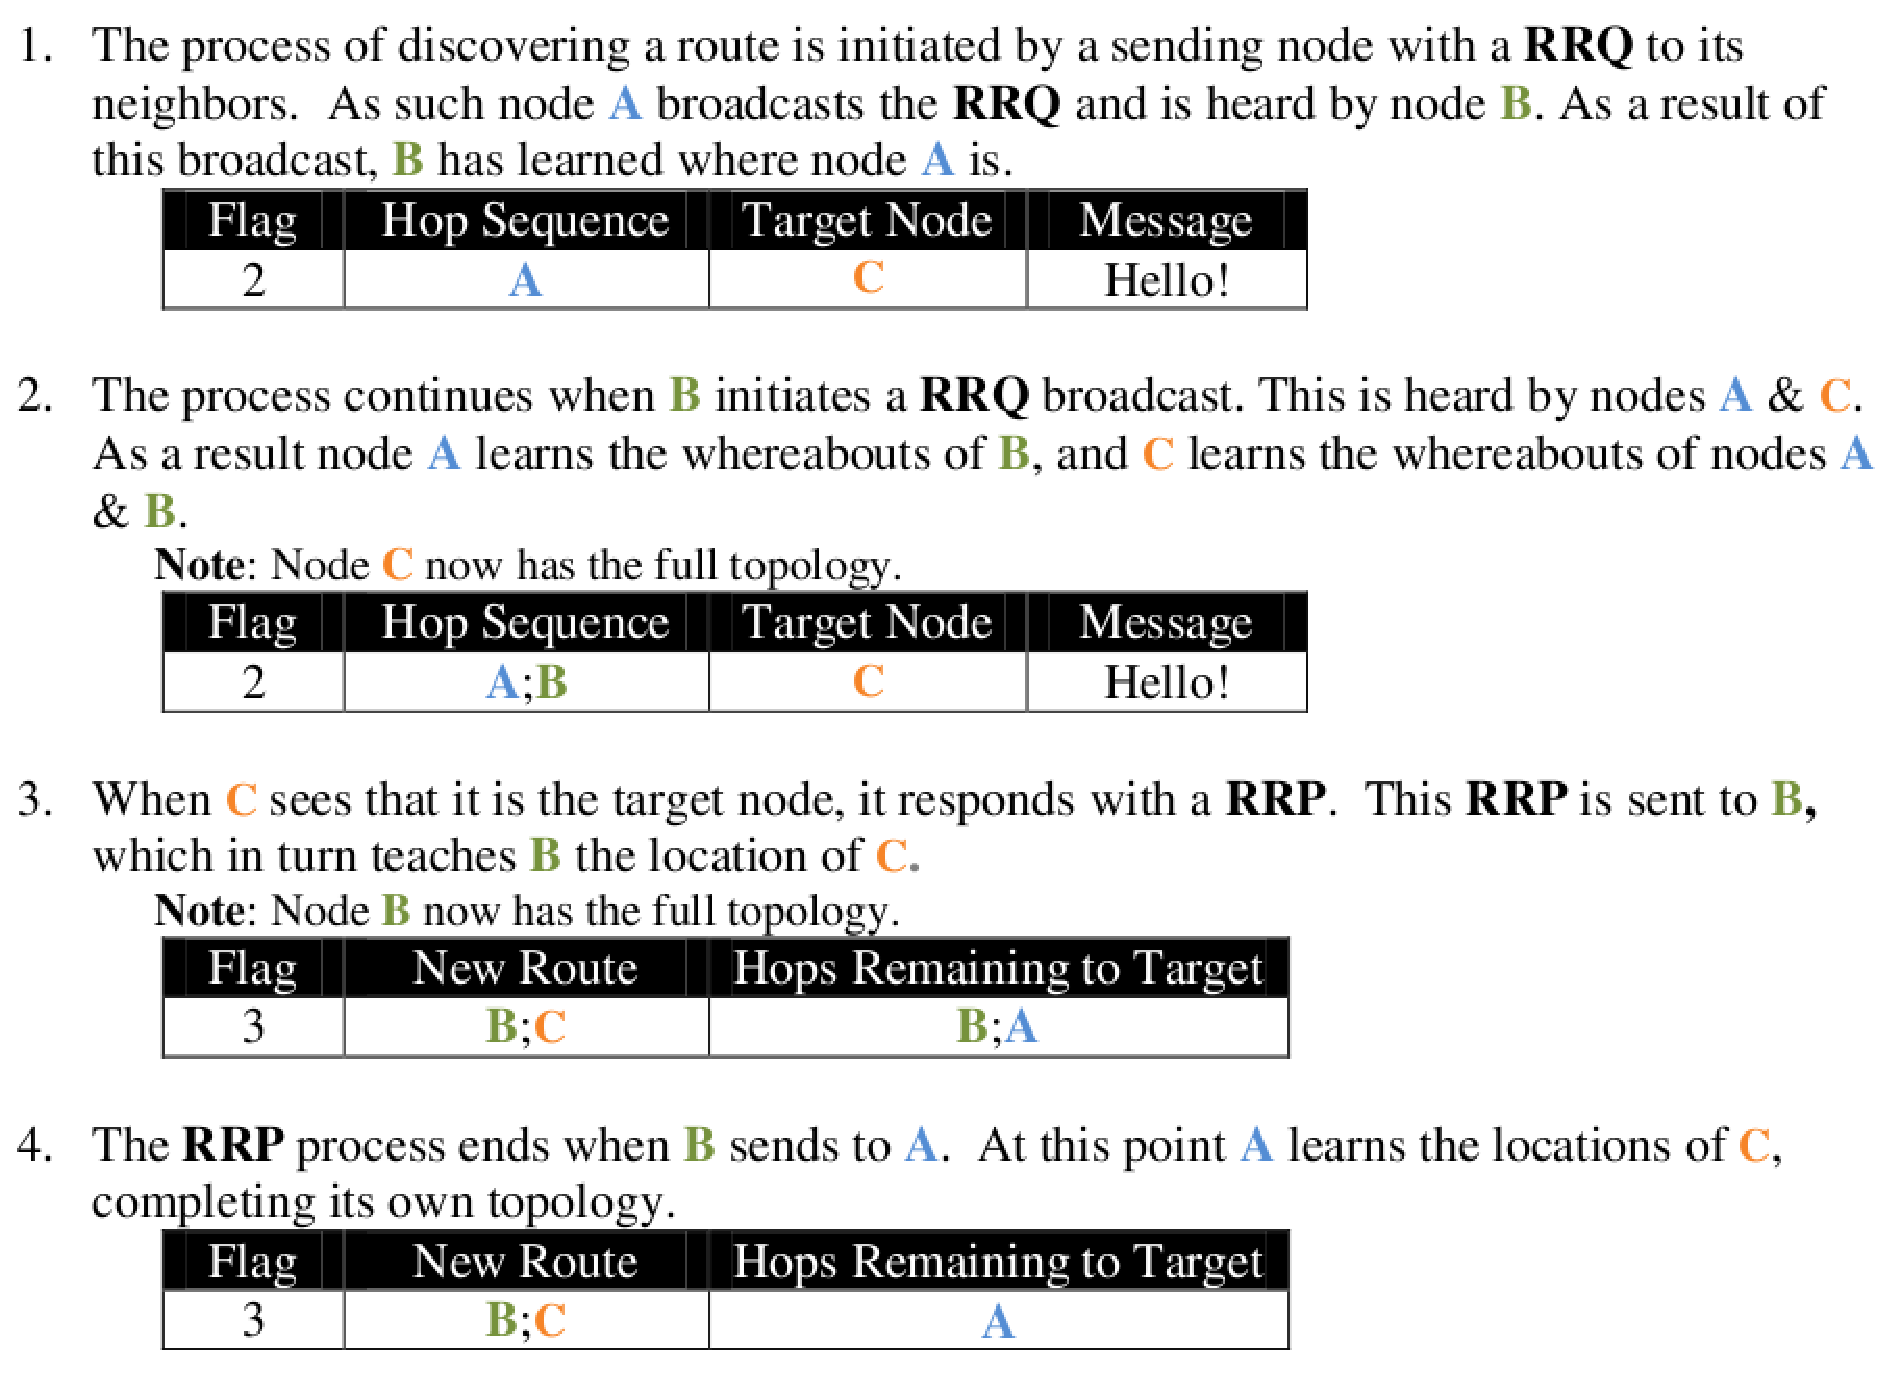
\includegraphics[scale=.5]{RRQ_RRP_A}
  \label{RRA}
\end{figure}

\subsection*{The Process of Sending Data}

\begin{figure}[!h]
  \centering
  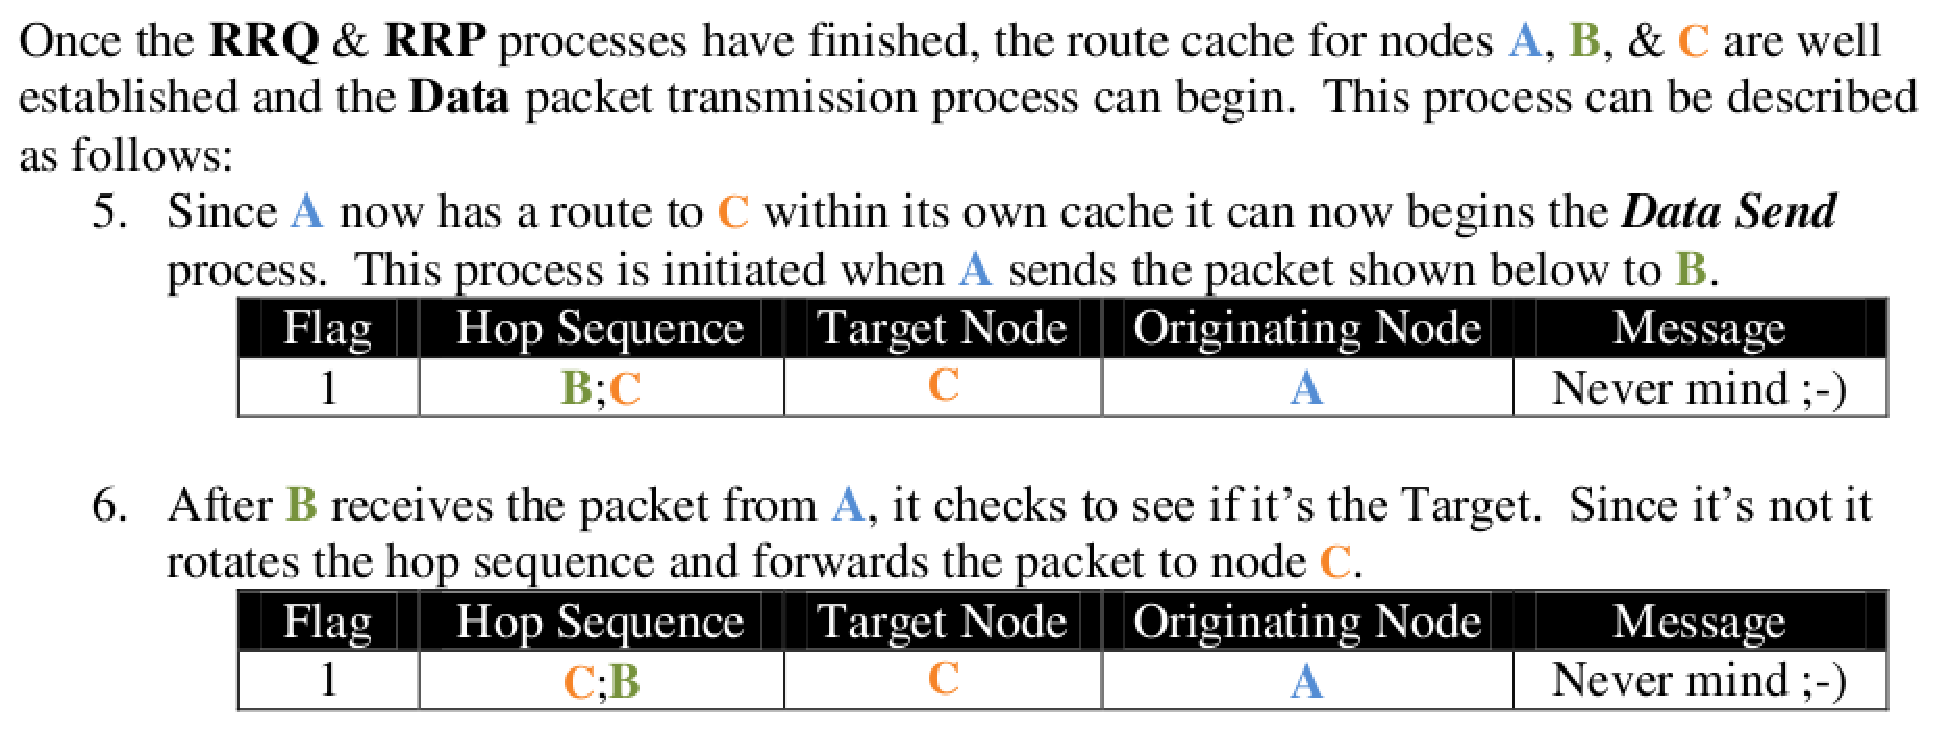
\includegraphics[scale=.5]{RRQ_RRP_B}
  \label{RRB}
\end{figure}

\begin{figure}[!h]
  \centering
  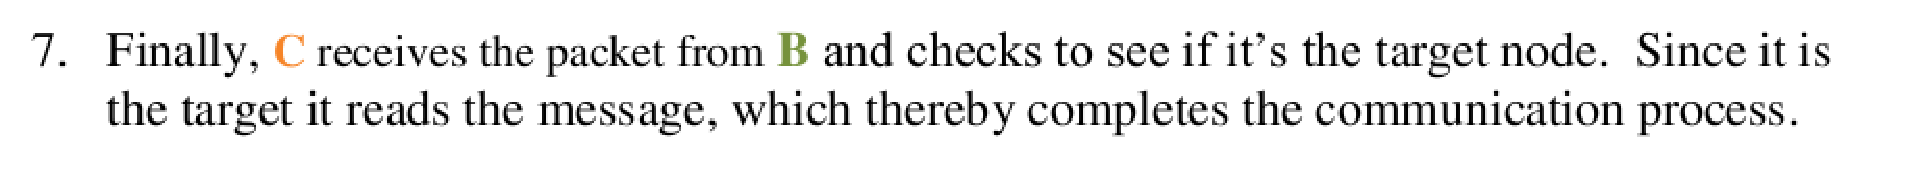
\includegraphics[scale=.5]{RRQ_RRP_C}
  \label{RRB}
\end{figure}

\section{Performance Evaluation and Results}

Technical difficulties impeded our ability to properly evaluate the performance of our algorithm.  This is because not all of the Nokia N800’s devices were properly configured, and thus could not be utilized.  It was determined that since the only reason for originally using the N800’s was because of the initial desire to implement OLSR as a plug-in for the devices.  Otherwise, they were simply Linux-running tablets.  Therefore a “Plan B” for testing involved a combination of the tablets and Linux-running laptops.

Off-campus, an ad hoc network between the laptops and N800’s was successfully created.  The algorithm itself was verified as working.  Route discovery and message transmission worked successfully.  Another problem quickly became an obstacle, however; a “structured” topology could not be created due to the inability to use MAC filtering successfully.  At this point, time became an issue in making further progress in this area.

\section{Conclusion}

This project was an excellent project for understanding, designing, and implementing a Dynamic Source Routing algorithm.  Everyone was able to actively and effectively contribute to the design of the project.  This was the most important part in terms of actually understanding what DSR is and how it works.  This well-planned design turned into a fundamentally functional application with demonstrated success.  

Unfortunately, two key factors contributed to us having to “end” the project where we did.  The first was the difficulties with the N800’s.  This includes the large amount of time spent on trying to comprehend the plug-in aspect of the tablets before ultimately dismissing that option and going for a standalone application.  Afterwards, the time spent before determining that not all of the tablets were properly configured for our use.  Ultimately, this lead to our second and biggest issue: simple time constraint.  While there was enough time to successfully design and implement a functioning DSR application, there simply was not enough time to do everything we had hoped to do. In terms of coding, all of diagram was implemented except for error handling.  This did give us enough functionality to proceed with performance evaluation/testing, had it not been for the other technical issues with the devices.

In the end, however, we are still satisfied with this DSR implementation.  We feel confident that our underlying algorithm works and believe that with a little more time and minus the time spent on OLSR, plugins, and technical difficulties, we would have been able to fully implement our design.  All-in-all, this was an enjoyable project that we were able to learn a great deal from.

\end{document}
